\documentclass[../main.tex]{subfiles}

\begin{document}
\subsection{Variations on Boxplots}

While bar graphs and histograms can give a sense of the variability in data, they are limited to showing the dispersion of the data only in how the measurements are spread out. This is somewhat limiting for very large datasets, so the box plot has evolved as a way to display more characteristics of the distribution \cite{wickham_40_2011}. 

\begin{figure}
  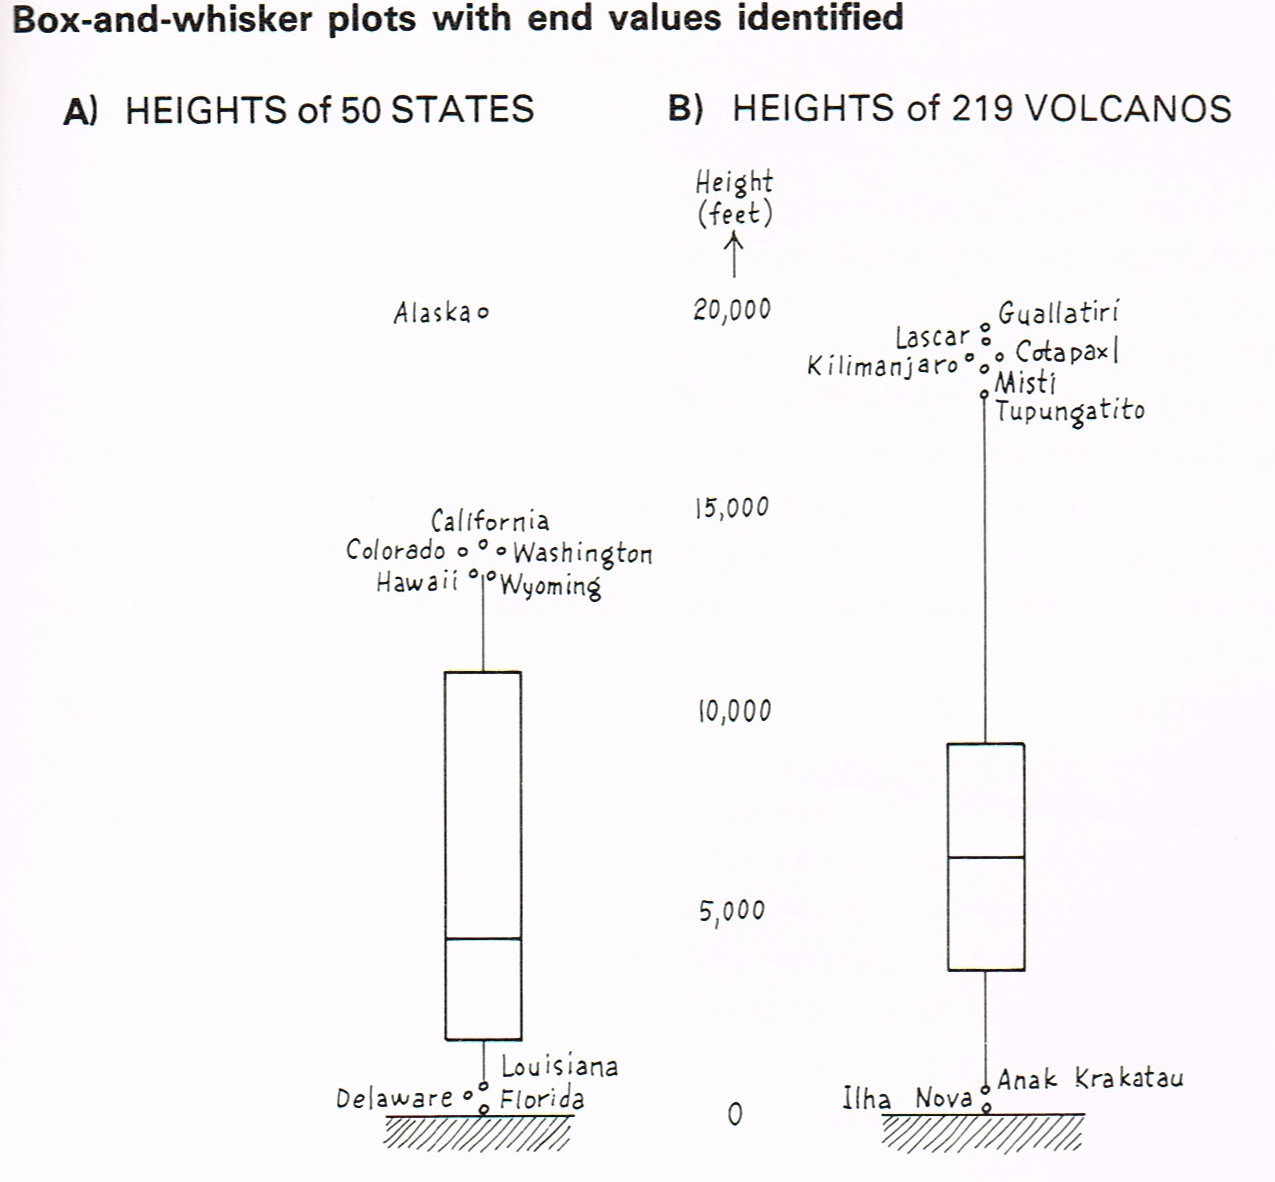
\includegraphics{boxplot}
  \caption{Tukey's 1977 example of the box plot from
    The box plot shows the distribution of topology of states and
    the distribution of volcanoes. The strength of the box and whisker is that the
    reader can quickly compare the two distributions and learn, for example,
    that volcanoes tend to span a shorter range of average heights, but that the
    extremes are much further from the center. Essentially, the distributions act as references for the other displayed distributions. Figure is from Exploratory Data Analytics\cite{tukey_exploratory_1977} }
  \label{fig:boxplot}
\end{figure}

Tukey's introduction to the box-plot \cite{tukey_exploratory_1977}, shown in
Figure~\ref{fig:boxplot} illustrates how the distributions of these 1 dimensional densities differ by category. While this graph shows the median, range between upper and lower interquartile, and lower and upper extreme, many authors have exploited the structure to convey more information about the data. Authors used different quantile levels \cite{hyndman_sample_1996}s or measures of outliers
\cite{frigge_implementations_1989, schwertman_identifying_2007}, or otherwise incorporated skewness, kurtosis, and other descriptive distributional statistics \cite{kim_more_2004, marmolejo-ramos_shifting_2015}.

\subsubsection{Boxplots for Curves}
While box plots were designed to visualize discrete observations, often there
are no discrete observations and instead the `observation` is a functional densities, drawn from a continuous sample of observations \cite{ramsay_functional_2006, muller_functional_2006}.
One such example is a timeseries curve (where the connections are as important as the individual points) or
spatial region. Understanding the distributions of functional observations
often relies first ordering the functions such that there's some measure of how close these functions are to each other--depth\cite{febrero_functional_2007,lopez-pintado_functional_2007},
bivariate score depth\cite{rob_j._hyndman_rainbow_2010}, and
bivariate kernel density estimation\cite{scott_multivariate_1992} are some examples. This
ordering then yields functional analogs to median and other percentile
metrics. For small values, the ordered curves can then be colored based on the
ordering metric \cite{rob_j._hyndman_rainbow_2010}, but this method is unwieldy for larger
ensembles.


\begin{figure}
  \begin{subfigure}{\textwidth}
    \centering
    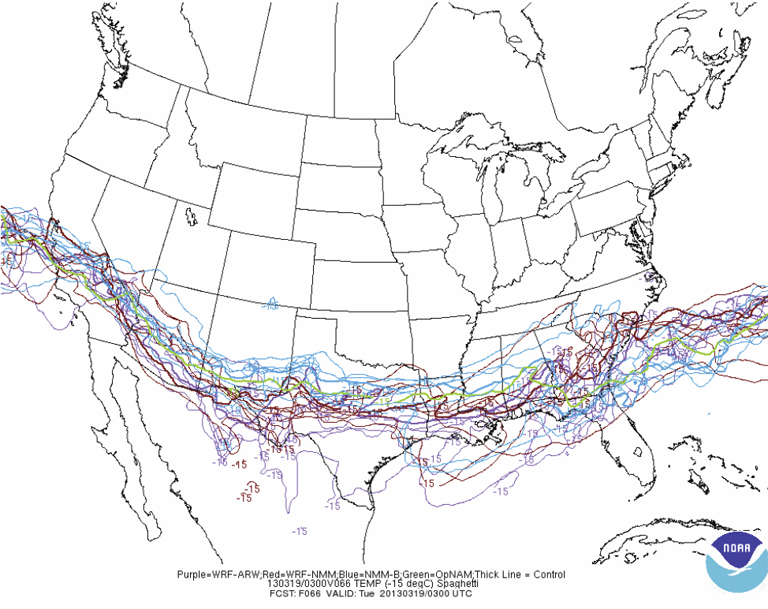
\includegraphics[scale=0.8]{spaghetti}
    \caption{Spaghetti plot of ensemble of 500mb and -15C temperature isocountours.}
    \label{fig:spaghetti}
    \end{subfigure}

    \bigskip
    \begin{subfigure}{\textwidth}
    \centering
    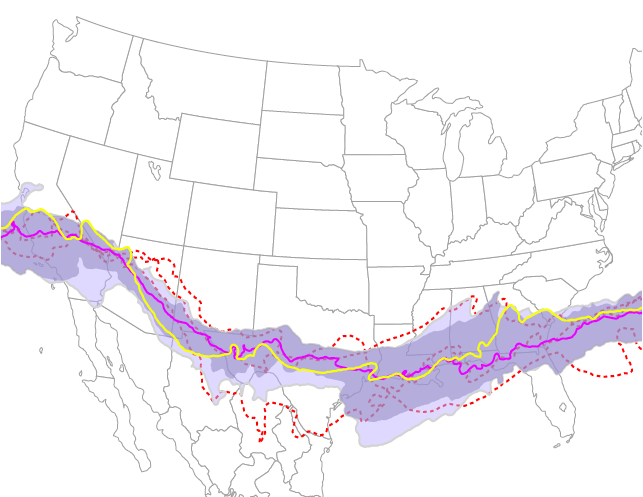
\includegraphics[scale=0.5]{contour_weather}
    \caption{This countour boxplot is showing the distribution of a temperature field at 500mb and -15C. The mean field is in yellow, the median in purple, red as outlier cut offs, and envelops for the minimum and maxmimum bands.}
    \label{fig:contour}
    \end{subfigure}
    \caption{Both figures are from Contour boxplots: A method for characterizing uncertainty in feature sets from simulation ensembles\cite{whitaker_contour_2013}}
\end{figure}

Functional bag, box, and HDR plots \cite{rob_j._hyndman_rainbow_2010, sun_functional_2011} tend to be good at visualizing specific types of outliers, but are somewhat limited in the variability they show. A very common task is to compare ensembles, each a function of the same timeseries or geographic region. Contour box plots\cite{whitaker_contour_2013} aim to capture the variability of the
uncertainty via a band depth ordering metric. Each ensemble members band depth
is computed as sum of the probabilities that the observations in any given
ensemble fall within the max-min envelope defined by any two other
ensembles. The bands are then sorted by band depth such that the median is the
ensemble with about 50\% of its members whiten all envelopes formed by other
bands (so most centered). Outer bands are chosen according to the task at
hand, which in this paper is temperature visualizations. As illustrated by figure~\ref{fig:spaghetti}, contour boxplots are an improvement over spaghetti plots \cite{luo_visualizing_2003, whitaker_contour_2013} because a lot of the nosiness is filtered out.  In figure~\ref{fig:countour}, the authors remove most of the bands and instead visualize an outlying envelope(light gray) and a more central envelope(dark gray). It retains much of the information of the spaghetti plot in figure~\ref{fig:spaghetti}, but removes the visual noise of the lines.

\subsubsection{Boxplots for Surfaces}
\begin{figure}
  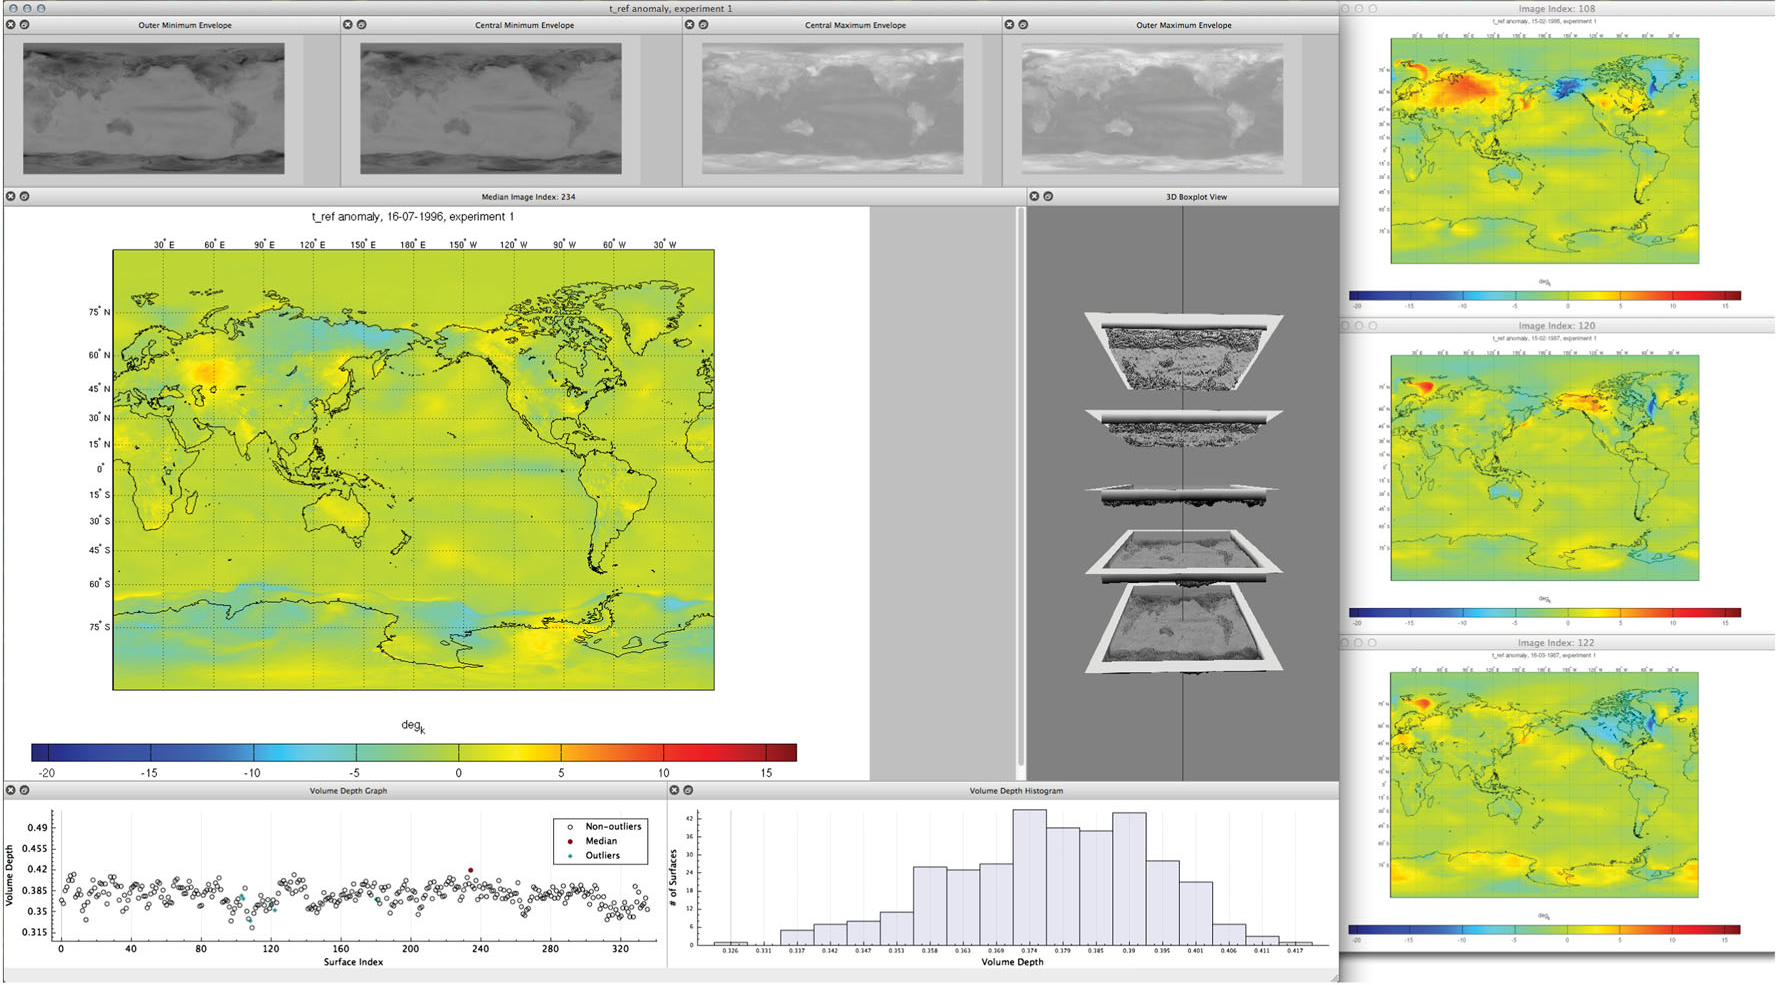
\includegraphics[width=1\linewidth]{surfacebox.png}
  \caption{The large colored surface in the middle is the median surfac. The surfaces on top are minimum and maximum envelopes. The graphs at the bottom visualize the distribution of band-depths of surfaces. The 3 surfaces on the right have been identified as outliers by the tool. This figure is from Surface boxplots \cite{genton_surface_2014}}
  \label{fig:surface}
\end{figure}
Another application of this band depth concept is to surfaces such as collections of images or functional data generated by models. In figure~\ref{fig:surface}, Genton et al. built a surface boxplot visualization tool with multiple panes\cite{genton_surface_2014}. Like a traditional boxplot, they display the median surface from the dataset, minimum and maximum surfaces, and they have a 3D view that gives a sense of how surfaces are distributed. The tool also provides histograms of the band depth to give a 2d view on how the surfaces are distributed.


\end{document}